\documentclass[../main.tex]{subfiles}
\graphicspath{{\subfix{../img/}}}
\begin{document}


\newpage
\section{HardwareTest}

\subsection{Ultraschallsensor}
Als Ultraschalloption hat man den Typ HC-SR04 getestet. Dieser hat eine Reichweite von 2 cm bis 300 cm mit einer Genauigkeit von 3 mm. Der Sensor wird einmal an 5 V angeschlossen und der Trig Pin aktiviert die Messung. Der Echo Pin empfängt das, vom Trig ausgelöste, Signal. Der Zeitunterschied zwischen Trig und Echo ist dann mit der Schallgeschwindigkeit umgerechnet die Distanz. Mit einem Testaufbau ermittelt man die reale Präzision dieses Sensors (sieh Abbildung \ref{fig:Ultraschall1}).

\begin{figure}[h] % 'h' steht für here, was bedeutet, dass das Bild möglichst an dieser Stelle eingefügt wird
    \centering
    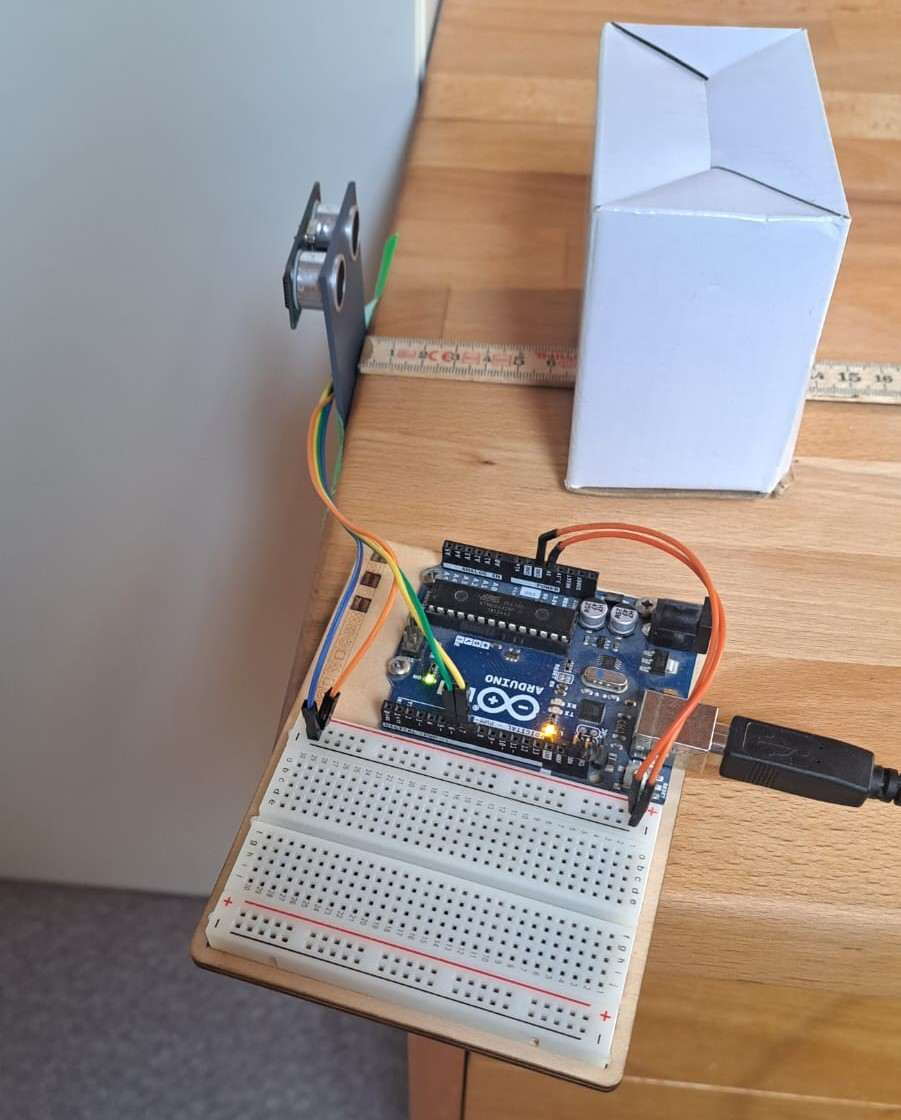
\includegraphics[width=0.5\textwidth]{img/sensortest/Ultraschall_Senkrecht.jpg} % Bildname und Breite der Grafik angeben
    \caption{Testaufbau Ultraschallsensor}
    \label{fig:Ultraschall1} % Label für die Referenzierung der Abbildung
\end{figure}

Daraus ergaben sich folgende Messwerte:
\begin{table}[H]
    \centering
    \begin{tabular}{cc} % zwei Spalten, zentriert ausgerichtet
        \textbf{Position} & \textbf{Messwert} \\ % Kopfzeile der Tabelle
        10 mm  & 25 mm  \\
        20 mm  & 24 mm  \\
        30 mm  & 29 mm  \\
        40 mm  & 42 mm  \\
        50 mm  & 51 mm  \\
        60 mm  & 59 mm  \\
        70 mm  & 71 mm  \\
        80 mm  & 79 mm  \\
        90 mm  & 86 mm  \\
        100 mm & 99 mm  \\
        110 mm & 105 mm \\
        120 mm & 113 mm \\
        130 mm & 129 mm \\
        140 mm & 139 mm \\
        150 mm & 150 mm \\
        160 mm & 163 mm \\
        170 mm & 169 mm \\
        180 mm & 184 mm \\
        190 mm & 190 mm \\
        200 mm & 199 mm \\
        210 mm & 210 mm \\
        220 mm & 219 mm \\
        230 mm & 225 mm \\
        240 mm & 237 mm \\
        250 mm & 250 mm \\
    \end{tabular}
    \caption{Tabelle der Positionen und Messwerte Ultraschall}
    \label{tab:messwerte}
\end{table}

Man sieht, dass der Sensor ungenauer ist in der Nähe des Sensors. Entfernt sich das Objekt, wird er präziser.

\newpage

\subsection{Time of Flight Sensor}
Ein Time of Flight Sensor funktioniert ähnlich wie ein Ultraschallsensor. Ausser das ein Lichtstrahl anstatt von einer Schallwelle ausgesendet wird. In diesem Versuch wird ein VL530LX verwendet. Der Testaufbau ist derselbe wie bei dem Ultraschallsensor (siehe Abbildung \ref{fig:TOF1}).

\begin{figure}[h] % 'h' steht für here, was bedeutet, dass das Bild möglichst an dieser Stelle eingefügt wird
    \centering
    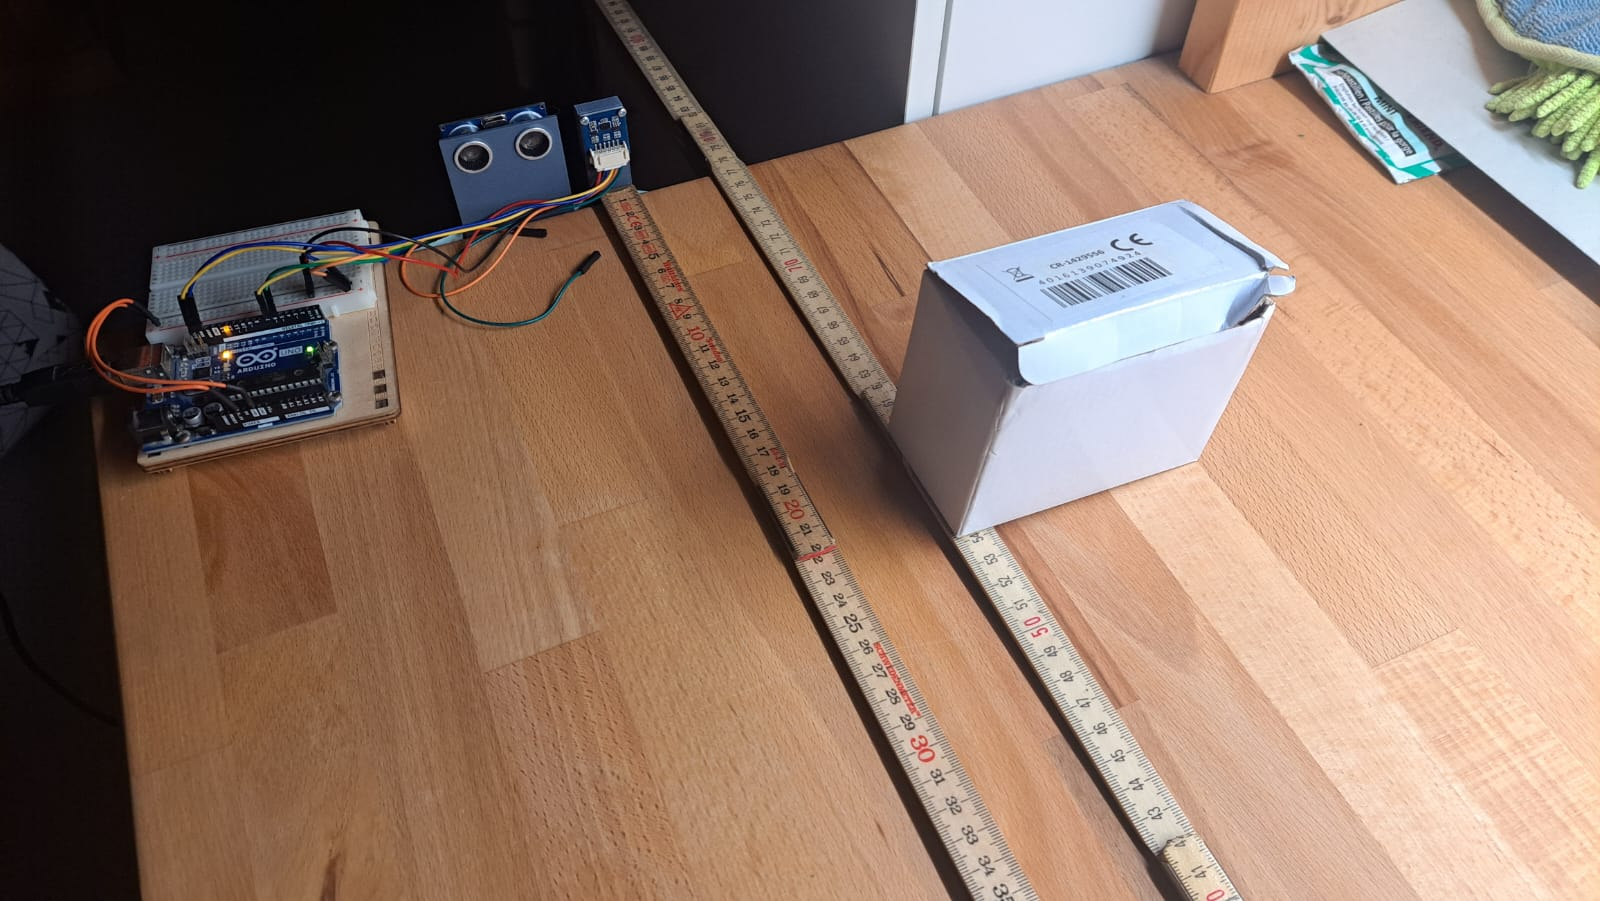
\includegraphics[width=0.5\textwidth]{img/sensortest/TOF_Verschoben.jpg} % Bildname und Breite der Grafik angeben
    \caption{Testaufbau TOF Sensor}
    \label{fig:TOF1} % Label für die Referenzierung der Abbildung
\end{figure}



Die Messungen ergaben folgende Resultate:


\begin{table}[H]
    \centering
    \begin{tabular}{cc} % zwei Spalten, zentriert ausgerichtet
        \textbf{Position} & \textbf{Messwert} \\ % Kopfzeile der Tabelle
        10 mm  & 18 mm  \\
        20 mm  & 22 mm  \\
        30 mm  & 30 mm  \\
        40 mm  & 43 mm  \\
        50 mm  & 52 mm  \\
        60 mm  & 61 mm  \\
        70 mm  & 73 mm  \\
        80 mm  & 82 mm  \\
        90 mm  & 94 mm  \\
        100 mm & 102 mm \\
        110 mm & 113 mm \\
        120 mm & 124 mm \\
        130 mm & 134 mm \\
        140 mm & 144 mm \\
        150 mm & 155 mm \\
        160 mm & 167 mm \\
        170 mm & 176 mm \\
        180 mm & 188 mm \\
        190 mm & 198 mm \\
        200 mm & 207 mm \\
        210 mm & 218 mm \\
        220 mm & 226 mm \\
        230 mm & 238 mm \\
        240 mm & 246 mm \\
        250 mm & 257 mm \\
    \end{tabular}
    \caption{Tabelle der Positionen und Messwerte TOF}
    \label{tab:messwerte}
\end{table}
Hier sieht man 


\end{document}